\chapter{Electric Dipole  and Dielectrics}

\section{Electric Dipole}
\begin{definition}
Electric dipole is a pair of equal and opposite charges, $+q$ and $-q$, separated by a very small distance. Total charge of the dipole is zero but electric field of the dipole is not necessarily zero as charges $q$ and $-q$ are
separated by some distance and electric field due to them when added is not zero.
\begin{figure}[H]
	\begin{center}
		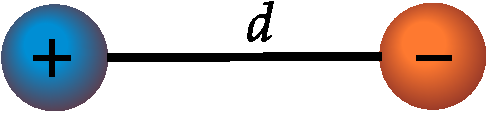
\includegraphics[width=0.25\textwidth]{dipole}
	\end{center}
\end{figure}
\end{definition}
\section{Electric Dipole moment}
 The dipole moment of an electric field is a vector whose magnitude is charge times the separation between two opposite charges.
Dipole moment for a collection of charges, $q_{i}$ having position vectors $\vec{r}_{i}$ is
\begin{equation}
$$
\vec{p}=\sum_{i} q_{i} \vec{r}_{i}
$$
\end{equation}

For continuous system the dipole moment is written as,
\begin{equation}
$$
\vec{p}=\int_{v} \vec{r} \rho(\vec{r}) d v
$$
\end{equation}

	$ \bullet $ \textbf{The dipole moment is independant of the choice of origin, if the monopole moment is zero.}


\begin{note}
	Monopole moment: Monopole moment is simply the sum of total charges of the system.
\end{note}
\begin{exercise}
Suppose three point charges $+\mathrm{q},+\mathrm{q},-2 \mathrm{q}$ place at the vertices of an equilateral triangle.
\end{exercise}
\begin{answer}
	Total charge of the system, $Q=+q+q-2 q=0$ \\
	$ \therefore $ dipole moment is independent of choice of origin. \\
	\begin{minipage}{0.40\textwidth}
		\begin{align*}
		\intertext{The dipole moment with respect to origin.}
		P&=q \times 0+q(a \hat{i})-2 q\left(\frac{a}{2} \hat{i}+\frac{\sqrt{3}}{2} a \hat{j}\right) \\
		&=0+q a \hat{i}-q a \hat{i}-q \sqrt{3} a \hat{j}\\&=-\hat{j} \sqrt{3} a q
		\end{align*}
	\end{minipage}\hfill
	\begin{minipage}{0.40\textwidth}
	\begin{figure}[H]
		\centering
		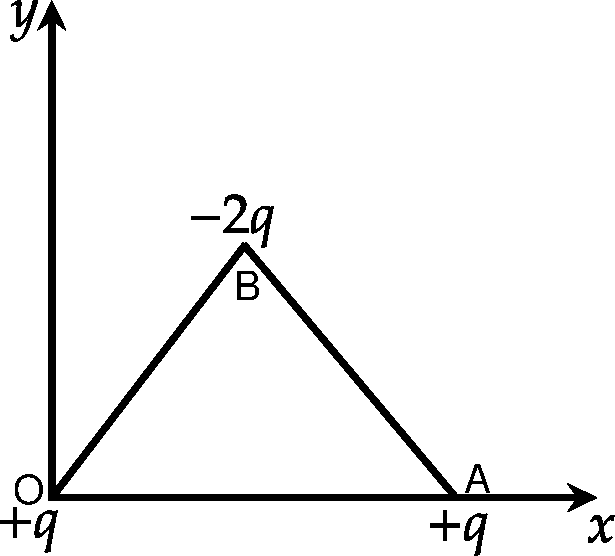
\includegraphics[height=4cm,width=4cm]{dipole1}
	\end{figure}
\end{minipage}

\end{answer}

\section{The Electric Potential and Field of a Dipole}
\begin{wrapfigure}{r}{0.20\textwidth}
	\begin{center}
		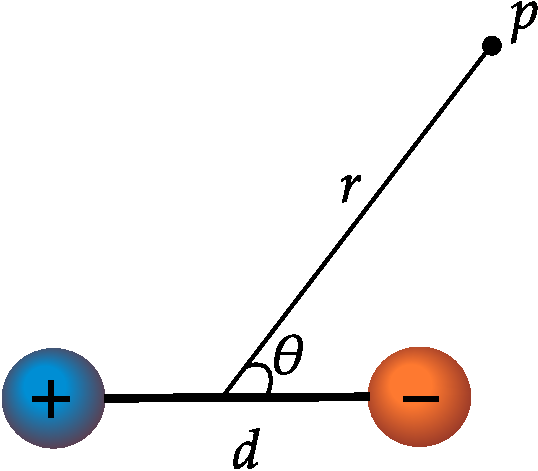
\includegraphics[width=0.20\textwidth]{dipole2}
	\end{center}
	\caption{electric dipole}
	\label{electric dipole}
\end{wrapfigure}

Consider a dipole as shown in the figure \ref{electric dipole}.
Let us calculate the electric potential and field caused by this dipole at an arbitrary point at a distance $r$ and at an angle $\theta$. Then it's Potential is given by,
\begin{equation}
$$
V_{\operatorname{dip}}({r,\theta})=\frac{1}{4 \pi \epsilon_{0}} \frac{{p} \cdot \hat{{r}}}{r^{2}}
=\frac{1}{4 \pi \epsilon_{0}} \frac{{p} \cos\theta}{r^{2}}
$$
\end{equation}
We know that $E=-\nabla V$
\\Then,to get the field, we take the negative gradient of $V$ :
\begin{align*}
E_{r}&=-\frac{\partial V}{\partial r}=\frac{2 p \cos \theta}{4 \pi \epsilon_{0} r^{3}} \\
E_{\theta}&=-\frac{1}{r} \frac{\partial V}{\partial \theta}=\frac{p \sin \theta}{4 \pi \epsilon_{0} r^{3}} \\
E_{\phi}&=-\frac{1}{r \sin \theta} \frac{\partial V}{\partial \phi}=0
\end{align*}
And then,
\begin{equation}
$$
\vec{E}_{\mathrm{dip}}(r, \theta)=\frac{p}{4 \pi \epsilon_{0} r^{3}}(2 \cos \theta \hat{{r}}+\sin \theta \hat{\boldsymbol{\theta}})
$$
\end{equation}
\begin{center}
	\framebox{
		\parbox[t][2.5cm]{7.5cm}{
			
			\addvspace{0.2cm} \centering 
			\begin{align*}
			V_{\operatorname{dip}}({r,\theta})&=\frac{1}{4 \pi \epsilon_{0}} \frac{{p} \cdot \hat{{r}}}{r^{2}}
			=\frac{1}{4 \pi \epsilon_{0}} \frac{{p} \cos\theta}{r^{2}}\\
			{E}_{\mathrm{dip}}(r, \theta)&=\frac{p}{4 \pi \epsilon_{0} r^{3}}(2 \cos \theta \hat{{r}}+\sin \theta \hat{\boldsymbol{\theta}})
			\end{align*}
			
		} }
\end{center}
\subsection{Variation of Potential and Field}
\begin{itemize}
	\item If total charge is non-zero(Monopole moment), then, $$V \propto \frac{1}{r}\quad ;\quad E \propto \frac{1}{r^{2}}$$
	\item If total charge is zero and dipole moment is non-zero, then, $$V \propto \frac{1}{r^{2}}\quad ;\quad E \propto \frac{1}{r^{3}}$$
	\item If total charge and dipole moment are zero and quadrupole term is non-zero then, $$V \propto \frac{1}{r^{3}}\quad ;\quad E \propto \frac{1}{r^{4}}$$
\end{itemize}
\begin{figure}[H]
	\begin{minipage}{0.24\textwidth}
		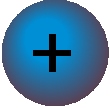
\includegraphics[width=0.25\textwidth]{monopole}
		\caption{Monopole}
	\end{minipage}
	\begin{minipage}{0.24\textwidth}
	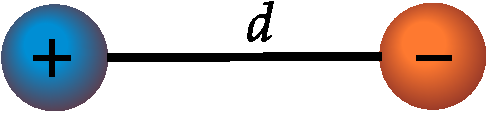
\includegraphics[width=0.65\textwidth]{dipole}
		\caption{Dipole}
	\end{minipage}
\begin{minipage}{0.24\textwidth}
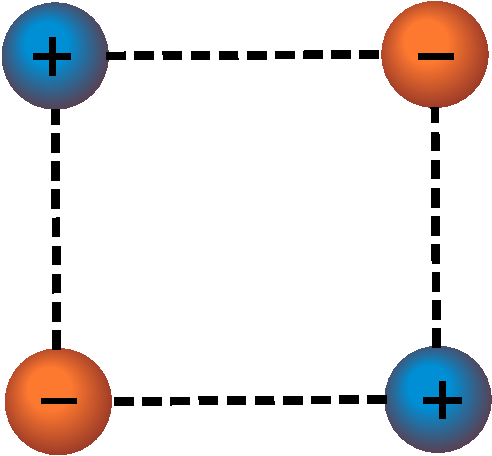
\includegraphics[width=0.65\textwidth]{quadrapole}
	\caption{Quadrapole}
\end{minipage}
\begin{minipage}{0.24\textwidth}
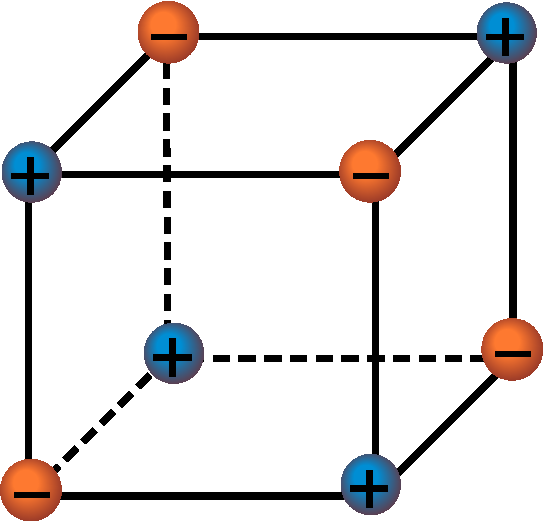
\includegraphics[width=0.65\textwidth]{octapole}
\caption{Octapole}
\end{minipage}
\end{figure}
\begin{exercise}
	An insulating sphere of radius $R$ carries a charge density
	$$
	\rho(\vec{r})=\rho\left(R^{2}-r^{2}\right) \cos ^{2} \theta ; \quad r<R
	$$
	Find the leading order term for the electric field at a distance $d$, far away from the charge
	distribution.
\end{exercise}
\begin{answer}
	\begin{align*}
	Q&=\int \rho d \tau=\rho \int\left(R^{2}-r^{2}\right) \cos ^{2} \theta \times r^{2} \sin \theta d r d \theta d \phi \neq 0 \\ &\Rightarrow V \propto \frac{1}{d} \Rightarrow E \propto \frac{1}{d^{2}}
	\end{align*}
	
\end{answer}
\section{Potential energy of a dipole placed in an external electric field}
Let we put a dipole whose $-q$ and $+$ q respectively at $\vec{r}$ and $(\vec{r}+\vec{d})$
The potential energy,
\begin{align*}
U&=-q V(\vec{r})+q V(\vec{r}+\vec{d})\\
U&=-q V(r)+q V(r)+q d \cdot \vec{\nabla} V(r)\quad \text{(using Taylor expansion)}\\
&=q d \cdot \vec{\nabla} V(r) \\
U&=\vec{p} \cdot \vec{\nabla} V(r) \\
U&=-\vec{p} \cdot \vec{E}(r) \quad(\because E(r)=-\nabla V(r))
\end{align*}
\subsection{Force and torque on a dipole placed in an electric field:}
\subsubsection{Force }
We know that,
\begin{align*}
\vec{F} &=-\vec{\nabla} U=\nabla(\vec{p} \cdot \vec{E}) \\
&=(\vec{p} \cdot \vec{\nabla}) \vec{E}+(\vec{E} \cdot \vec{\nabla}) \vec{p}+\vec{p} \times(\vec{\nabla} \times \vec{E})+\vec{E} \times(\vec{\nabla} \times \vec{p}) \\
&=(\vec{p} \cdot \vec{\nabla}) \bar{E}+0+0+0\\
\text{For uniform } \vec{E},\\
\vec{F}&=(\vec{p} \cdot \vec{\nabla}) \vec{E}=0
\end{align*}

that means there have no translational motion.
\subsubsection{Torque}
We know the potential energy of the dipole due external electrie field is $u=\vec{p} \cdot \vec{E}=p E \cos \theta$
Therefore, the torque about its own centre is
$$
\begin{aligned}
&\tau=-\frac{d u}{d \theta}=p E \sin \theta\\
&\text { Or, }\\
&\vec{\tau}=\vec{p} \times \vec{E}
\end{aligned}
$$
\textbf{Torque on the dipole in non-uniform electric field :}\\
The torque on a small dipole about its own centre is still
$$
\vec{\tau}=\vec{p} \times \vec{E}
$$
But since there is a net force $\vec{F}$ on the dipole.
Therefore, an extra torque act on the dipole is $\vec{r} \times \vec{F}$ about any other point.
Therefore, totaltorque about any other point is $\vec{\tau}=\vec{p} \times \vec{E}+\vec{r} \times \vec{F}$\\
\textbf{Mutual potential energy between two coplanar dipoles:}\\
Let consider two diple of dipole moment $\vec{p}_{1}$ and $\vec{p}_{2}$ lying on a single plane, $\vec{r}_{21}$ is the position vector of dipole
2 with respect to 1 . The electric field at the centre of dipole 2 is,
$$
\vec{E}_{1}=\frac{1}{4 \pi \varepsilon_{0}}\left[\frac{3\left(\vec{p}_{1} \cdot \vec{r}_{21}\right) \vec{r}_{21}}{r_{21}^{5}}-\frac{\vec{p}_{1}}{r_{21}^{3}}\right]
$$
The mutual potential energy,
$$
U_{21}=-\vec{p}_{2} \cdot \vec{E}_{1}=-\vec{p}_{1} \cdot \vec{E}_{2}=\frac{1}{4 \pi \varepsilon_{0}}\left[\frac{\vec{p}_{1} \cdot \vec{p}_{2}}{r_{21}^{3}}-\frac{3\left(\vec{p}_{1} \cdot \vec{r}_{21}\right)\left(\vec{p}_{2} \cdot \vec{r}_{21}\right)}{r_{21}^{5}}\right]
$$

\section{Dielectrics}
Insulators or Dielectrics is a different class of material from which we have been discussing till now. The primary difference between a conductor and a dielectric is that in the dielectrics, the electric charges (primarily the valence electrons)   which could be free in conductors are tightly bound to the parent atoms or molecules. The dielectric materials are made up of either 'polar molecules' or 'non- polar molecules'.\\
\begin{minipage}{0.60\textwidth}
	\subsubsection{Polar molecules}
	In polar molecules there always exists a seperation between average positions of positive and negative charges. It has a net permanent dipole as a result of opposing charges due to asymmetrical bonds.
	\begin{example}
		Water ($ H_{2}O $), Ammonia ($ NH_{3} $), and Ozone ($ O_{3} $)
	\end{example}  
\end{minipage}\hfil
\begin{minipage}{0.30\textwidth}
	\begin{figure}[H]
		\centering
		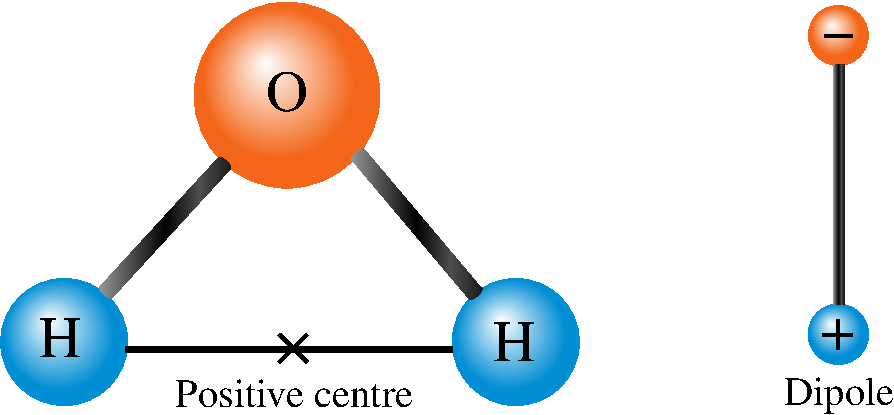
\includegraphics[height=3cm,width=6.5cm]{watermolecule}
		\caption{ Water molecule , $H_{2}O$}
		\label{}
	\end{figure}
\end{minipage}\\
\begin{minipage}{0.60\textwidth}
	\subsubsection{Non-Polar molecules}
	The molecule in which the centre of gravity of molecule coincide  with electrons are known as non-polar molecules they don't have permanent dipole moment .
	\begin{example}
		Hydrogen ($ H_{2} $), Oxygen ($ O_{2} $), and Carbon dioxide ($ CO_{2} $)
	\end{example} 
\end{minipage}\hfil
\begin{minipage}{0.30\textwidth}
	\begin{figure}[H]
		\centering
		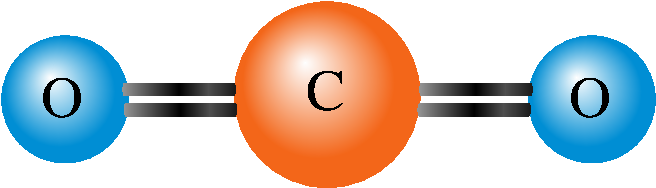
\includegraphics[height=1cm,width=3.5cm]{carbon dioxide}
		\caption{Carbon dioxide molecule , $CO_{2}$}
		\label{}
	\end{figure}
\end{minipage}
\subsection{Dielectric Polarization} 
When a dielectric is subjected to an electric field, the electrons do not wander around but respond to such a field in a different way. 
The response of dielectrics to an applied electric field are of two different kinds. In what are known as "polar molecules", even in the absence of an electric field the charge centres for positive and negative charges do not coincide. This results in the molecules developing a permanent dipole moment. In "non-polar molecules", in the absence of an electric field, the positive and the negative charge centres coincide and there is no dipole moment. However, when an electric field is applied, there is a charge separation and a dipole moment is induced. The induced dipole moment vanishes once the electric field is withdrawn.

\begin{minipage}{0.45\textwidth}
	\begin{figure}[H]
		\centering
		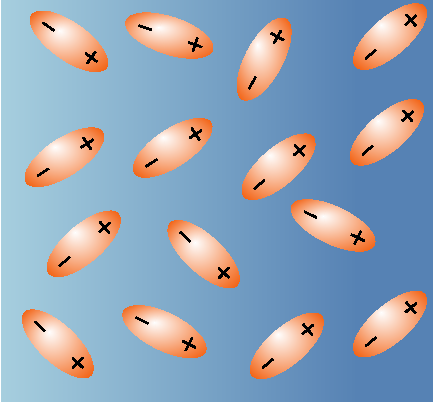
\includegraphics[height=4cm,width=5cm]{polarization 1}
		\caption{Polar molecules of dielectric in the absence of electric field ($\vec{E}=0$).}
		\label{}
	\end{figure}
\end{minipage}\hfil
\begin{minipage}{0.45\textwidth}
	\begin{figure}[H]
		\centering
		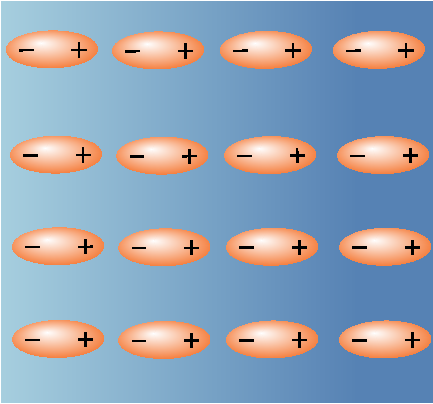
\includegraphics[height=4cm,width=5cm]{polarization 2}
		\caption{Polar molecules of dielectric in the presence of electric field ($\vec{E}\neq 0$).}
		\label{}
	\end{figure}
\end{minipage}
\\\\\\Dielectric polarization occurs when a dipole moment is formed in an insulating material because of an externally applied electric field. When a current interacts with a dielectric (insulating) material, the dielectric material will respond with a shift in charge distribution with the positive charges aligning with the electric field and the negative charges aligning against it. A convenient maeasure of this is the \textbf{polarization},
$$\vec{ P} \equiv \text{Dipole moment per unit volume}=\lim _{\Delta V \rightarrow 0} \frac{1}{\Delta V} \sum_{i} \vec{p}_{i}$$
\subsection{Bound Charges}
Suppose we have a piece of polarized material that is, an object cotaining a lot of microscopic dipoles lined up. The dipole moment per unit volume $P$ (polarization) is given, 
\begin{figure}[H]
	\centering
	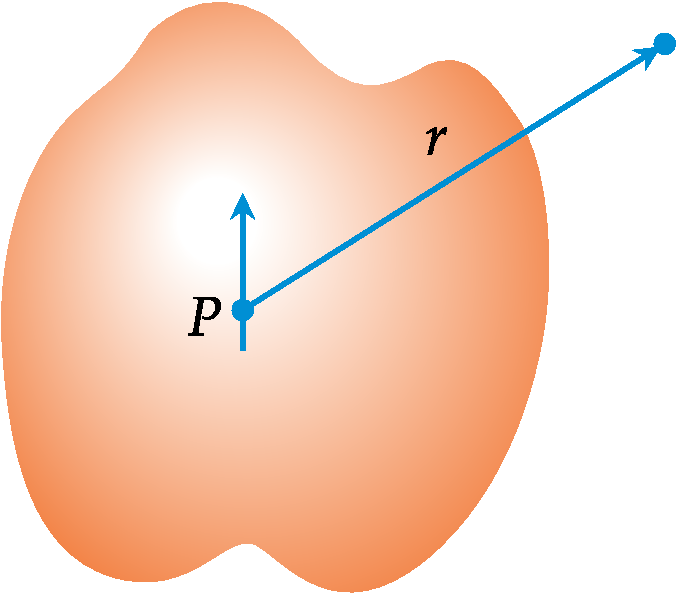
\includegraphics[height=4cm,width=4cm]{diagram-20220208(11)-crop}
\end{figure}
To find the field produced by this polarized object chop the material into infinitesimal dipoles and integrate to get the total. Since it's easier to deal with potential.\\
For a single dipole $P$\\
$$V(\mathbf{r})=\frac{1}{4 \pi \epsilon_{0}} \frac{\mathbf{p} \cdot \hat{\imath}}{\imath^{2}}$$
Dipole mom                                                                                                                                                                                                                                                                                                                                                                                                                                  ent $\mathbf{p}=\mathbf{P} d \tau^{\prime}$ in each volume element $d \tau^{\prime}$, so the total potential is
$$
V(\mathbf{r})=\frac{1}{4 \pi \epsilon_{0}} \int_{\mathcal{V}} \frac{\mathbf{P}\left(\mathbf{r}^{\prime}\right) \cdot \hat{\imath}}{r^{2}} d \tau^{\prime}
$$
Observing that,
$$\nabla^{\prime}\left(\frac{1}{r}\right)=\frac{\hat{\imath}}{r^{2}}$$
where  the differentiation is with respect to the source coordinates $\left(\mathbf{r}^{\prime}\right)$, we have
$$
V=\frac{1}{4 \pi \epsilon_{0}} \int_{\mathcal{V}} \mathbf{P} \cdot \nabla^{\prime}\left(\frac{1}{r}\right) d \tau^{\prime}
$$
Integrating by parts,  gives
$$
V=\frac{1}{4 \pi \epsilon_{0}}\left[\int_{\mathcal{V}} \nabla^{\prime} \cdot\left(\frac{\mathbf{P}}{r}\right) d \tau^{\prime}-\int_{\mathcal{V}} \frac{1}{r}\left(\nabla^{\prime} \cdot \mathbf{P}\right) d \tau^{\prime}\right]
$$
or, invoking the divergence theorem,
$$
V=\frac{1}{4 \pi \epsilon_{0}} \oint_{\mathcal{S}} \frac{1}{r} \mathbf{P} \cdot d \mathbf{a}^{\prime}-\frac{1}{4 \pi \epsilon_{0}} \int_{\mathcal{V}} \frac{1}{r}\left(\nabla^{\prime} \cdot \mathbf{P}\right) d \tau^{\prime}
$$
The first term looks like the potential of a surface charge
$$
\sigma_{b} \equiv \mathbf{P} \cdot \hat{\mathbf{n}}
$$
(where $\hat{\mathbf{n}}$ is the normal unit vector), while the second term looks like the potential of a volume charge
$$
\rho_{b} \equiv-\nabla \cdot \mathbf{P}
$$
$V(\mathbf{r})=\frac{1}{4 \pi \epsilon_{0}} \oint_{\mathcal{S}} \frac{\sigma_{b}}{r} d a^{\prime}+\frac{1}{4 \pi \epsilon_{0}} \int_{\mathcal{V}} \frac{\rho_{b}}{r} d \tau^{\prime}$
What this means is that the potential (and hence also the field) of a polarized object is the same as that produced by a volume charge density $\rho_{b}=-\boldsymbol{\nabla} \cdot \mathbf{P}$ plus a surface charge density $\sigma_{b}=\mathbf{P} \cdot \hat{\mathbf{n}}$. 
\section{The Electric Displacement}

\subsection{Gauss law in the presence of Dielectrics}
Effect of polarization is to produce accumulations of (bound) charge, $\rho_{b}=-\nabla\cdot P$ within the dielectric and $\sigma_{b}=P\cdot \hat{n}$ on the surface. The field due to polarization of the medium is just the field of this bound charge.  The total field will be the field attributable to bound charge plus the field due to free charge.\\
Free charge: any charge, that is not a result of polarization.\\
eg: electrons on a conductor\\
ions embedded in the dielectric material.

 Within the dielectric, then, the total charge density can be written:
 \begin{align*}
\rho&=\rho_{b}+\rho_{f} \\
\rho_{b}&=\text{Bound charge} \ \text{And}\ \rho_{f}= \text{Free charge} 
 \end{align*}
 By Gauss law,
 $\boldsymbol{\nabla} \cdot \vec{E}=\frac{\rho}{\epsilon_{0} }\Longrightarrow  \epsilon_{0}\boldsymbol{\nabla} \cdot \vec{E} =\rho_{b}+\rho_{f}=-\boldsymbol{\nabla} \cdot {P}+\rho_{f}$
 \\\\Where $\vec{E}$ is now the total field, not just that portion generated by polarization. It is convenient to combine the two divergence terms,
 $$
 \boldsymbol{\nabla} \cdot\left(\epsilon_{0} \vec{E}+\vec{P}\right)=\rho_{f}
 $$
 The expression in parentheses, designated by the letter ${D}$,
 \begin{center}
 	\framebox{
 		\parbox[t][1cm]{4cm}{
 			
 			\addvspace{0.2cm} \centering 
 			
 			$\vec{D} \equiv \epsilon_{0} \vec{E}+\vec{P}$} }
 \end{center}
  
 Is known as the \textbf{electric displacement}. In terms of ${D}$, Gauss's law becomes,
 $$
{\boldsymbol{\nabla} \cdot\vec{D}=\rho_{f}}
 $$
In integral form,
 $$
 \oint \vec{D} \cdot d{a}=Q_{f_{\mathrm{enc}}}
 $$
 \subsection{Linear Dielectrics}
 We define a linear dielectric as one where the polarization at a point in the dielectric  is proportional to the  electric field at the point. Provided ${\vec{E}}$ is not too strong: $$\vec{P} \propto \vec{E} \Rightarrow \vec{P}=\varepsilon_{0} \chi_{e} \vec{E}$$
 Materials that obey this relation are called linear dielectrics.\ $\chi_{e}$ is called the \textbf{electric susceptibility of the medium}.\\
 In linear media we have
 \begin{align*}
\vec{D}&=\varepsilon_{0} \vec{E}+\vec{P}=\varepsilon_{0} \vec{E}+\varepsilon_{0} \chi_{e} \vec{E}\\&=\varepsilon_{0} \vec{E}\left(1+\chi_{e}\right)=\varepsilon \vec{E} \\\text { Where ,}\  \varepsilon&=\varepsilon_{0}\left(1+\chi_{e}\right)
 \end{align*}
 This new constant $\varepsilon$ is called the \textbf{permittivity of the material}.\\
 $\varepsilon_{0}$ is permittivity of free space
 $$\varepsilon_r=1+\chi_{e}=\frac{\varepsilon}{\varepsilon_{0}}$$
 $\varepsilon_r$ \textbf{relative permittivity} or dielectric constant.\\
 Linear dielectric escape the defect in the parallel between $\vec{E}$ and $\vec{D}$ Since 
 $$ \vec{ P}\propto \vec{E} \quad\text{and}\quad\vec{ D}\propto \vec{E} ,$$
 It does not mean that 
 $$\vec{\nabla}\times \vec{P}=0 \text{ or }\vec{\nabla}\times \vec{ D}=0 \text{ when }\vec{ \nabla}\times \vec{E}=0$$\\
 The line integral of $\vec{P}$ around a closed path that straddles the boundary between one type of material and another need not be zero, even though the integral of $\vec{E}$ around the same loop must be.The reason is that the proportionality factor $\in_{0}\chi_{e}$ is different on on the two sides.\\\\
 \begin{itemize}
 	\item The space is entirely filled with a \textbf{homogeneous linear dielectric},
 \end{itemize}
$$\boldsymbol{\nabla} \cdot \mathbf{D}=\rho_{f}\text{ and }\boldsymbol{\nabla} \times \mathbf{D}=\mathbf{0},$$
so $\mathbf{D}$ can be found from the free charge just as though the dielectric were not there:
$$
\mathbf{D}=\epsilon_{0} \mathbf{E}_{\mathrm{vac}}
$$
where $\mathbf{E}_{\text {vac }}$ is the field the same free charge distribution would produce in the absence of any dielectric.therefore,
$$
\mathbf{E}=\frac{1}{\epsilon} \mathbf{D}=\frac{1}{\epsilon_{r}} \mathbf{E}_{\mathrm{vac}} .
$$
\textit{ When all space is filled with a homogeneous linear dielectric, the field everywhere is simply reduced by a factor of one over the dielectric constant.}
 \subsection{Boundary conditions in $\vec{D}$}
 The boundary between two medium is a
 thin sheet of free surface charge $\sigma_{f}$.
 The Gauss's law states that
  \begin{align*}
  \oint_{S} \vec{E}\cdot d \vec{a}&=\frac{Q_{\text {free }}}{\epsilon_{0}} \qquad \because D= {\epsilon_{0}}E\\
  \oint_{S} \vec{D}\cdot d \vec{a}&=Q_{\text {free }} \Rightarrow D_{\text {above }}^{\perp}-D_{\text {below }}^{\perp}=\sigma_{f}\\
 \text{Since, }
 \vec{D}&=\varepsilon_{0} \vec{E}+\vec{P} \Rightarrow \vec{\nabla} \times \vec{D}\\&=\vec{\nabla} \times \vec{P}\\
 \Rightarrow \vec{D}_{a b o v e}^{\|}-\vec{D}_{b e l o w}^{\|}&=\vec{P}_{\text {above }}^{\|}-\vec{P}_{\text {below }}^{\|} \\
 (\because \vec{\nabla} \times \vec{E}&=0)
 \end{align*}
 \begin{center}
 	\framebox{
 		\parbox[t][2cm]{4cm}{
 			
 			\addvspace{0.2cm} \centering 
 			
 			$E_{\text {above }}^{\perp}-E_{\text {below }}^{\perp}=\frac{1}{\epsilon_{0}} \sigma$\vspace{0.5cm} 			$\mathbf{E}_{\text {above }}^{\|}-\mathbf{E}_{\text {below }}^{\|}=0$} }
 \end{center}
\textbf{Boundary conditions for Linear Dielectrics}\\\\
In a (homogeneous isotropic) linear dielectric, the bound charge density $\left(\rho_{b}\right)$ is proportional to the free charge density $\left(\rho_{f}\right)$
$$
\rho_{b}=-\nabla \cdot \mathbf{P}=-\nabla \cdot\left(\epsilon_{0} \frac{\chi_{e}}{\epsilon} \mathbf{D}\right)=-\left(\frac{\chi_{e}}{1+\chi_{e}}\right) \rho_{f} .
$$
\textit{Unless free charge is actually embedded in the material, $\rho=0$, and any net charge must reside at the surface.Here potential obeys Laplace's equation.}\\\\$\therefore$  boundary conditions will be
$$
\epsilon_{\text {above }} E_{\text {above }}^{\perp}-\epsilon_{\text {below }} E_{\text {below }}^{\perp}=\sigma_{f},
$$
in terms of the potential,
$$
\epsilon_{\text {above }} \frac{\partial V_{\text {above }}}{\partial n}-\epsilon_{\text {below }} \frac{\partial V_{\text {below }}}{\partial n}=-\sigma_{f},
$$
whereas the potential itself is continuous
$$
V_{\text {above }}=V_{\text {below }}
$$
\subsection{Electrostatic energy in dielectric}

$$
U=\frac{1}{2} \int(\vec{E} \cdot \vec{D}) d V
$$
Therefore, the energy density in dielectric, $$U=\frac{1}{2}(\vec{E} \cdot \vec{D})$$ 
\begin{exercise}
	 A metal sphere of radius $a$ carries a charge $Q .$ It is surrounded, out to radius $b$, by
	linear dielectric material of permittivity $\varepsilon$. Find the potential at the center.
\end{exercise} 
\begin{answer}
	 $\oint \vec{D} \cdot d \vec{a}=Q_{f_{e n c}} \Rightarrow \vec{D}=\frac{Q}{4 \pi r^{2}} \hat{r} ;$ for all points $r>a$\\
	(Inside the metal sphere, $\vec{E}=\vec{P}=\vec{D}=0$) . \\Once we know $\vec{D}$, it is a trivial matter to obtain
	$\vec{E}$ by $\vec{D}=\varepsilon \vec{E}) .$
	$$
	\vec{E}=\left\{\begin{array}{ll}
	\frac{Q}{4 \pi \varepsilon r^{2}} \hat{r} & \text { for } a<r<b \\
	\frac{Q}{4 \pi \varepsilon_{0} r^{2}} \hat{r} & \text { for } r>b \\
	0 & \text { for } r<a
	\end{array}\right.
	$$
	Potential at the center is therefore,
	\begin{align*}
	V&=-\int_{\infty}^{0} \vec{E} \cdot d \vec{l}\\&=-\int_{\infty}^{b}\left(\frac{Q}{4 \pi \varepsilon_{0} r^{2}}\right) d r-\int_{b}^{a}\left(\frac{Q}{4 \pi \varepsilon r^{2}}\right) d r-\int_{a}^{0}(0) d r \\\Rightarrow V&=\frac{Q}{4 \pi}\left(\frac{1}{\varepsilon_{0} b}+\frac{1}{\varepsilon a}-\frac{1}{\varepsilon b}\right)
	\end{align*}
	
\end{answer}
\newpage
\begin{abox}
Practise Set-1
\end{abox}
\begin{enumerate}[label=\color{ocre}\textbf{\arabic*.}]
	
	\item Two electric dipoles $P_{1}$ and $P_{2}$ are placed at (0,0,0) and (1,0,0) respectively with both of them pointing in the $+z$ direction. Without changing the orientations of the dipoles $P_{2}$ is moved to (0,2,0) . The ratio of the electrostatic potential energy of the dipoles after moving to that before moving is
	{\exyear{IIT JAM 2006}}
	\begin{tasks}(4)
		\task[\textbf{a.}] $\frac{1}{16}$
		\task[\textbf{b.}] $\frac{1}{2}$
		\task[\textbf{c.}] $\frac{1}{4}$
		\task[\textbf{d.}] $\frac{1}{8}$
	\end{tasks}
		\item In a parallel plate capacitor the distance between the plates is $10 \mathrm{~cm}$. Two dielectric slabs of thickness $5 \mathrm{~cm}$ each and dielectric constants $K_{1}=2$ and $K_{2}=4$ respectively, are inserted between the plates. A potential of $100 V$ is applied across the capacitor as shown in the figure. The value of the net bound surface charge density at the interface of the two dielectrics is {\exyear{IIT JAM 2014}}
	\begin{figure}[H]
		\begin{center}
			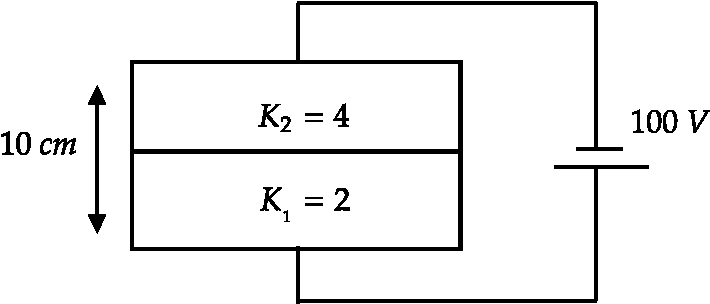
\includegraphics[width=0.30\textwidth]{EM-17(q)-crop}
		\end{center}
	\end{figure}
	\begin{tasks}(4)
		\task[\textbf{a.}] $-\frac{2000}{3} \varepsilon_{0}$
		\task[\textbf{b.}] $-\frac{1000}{3} \varepsilon_{0}$
		\task[\textbf{c.}] $-250 \varepsilon_{0}$
		\task[\textbf{d.}] $\frac{2000}{3} \varepsilon_{0}$
	\end{tasks}
	\item   A hollow, conducting spherical shell of inner radius $R_{1}$ and outer radius $R_{2}$ encloses a charge $q$ inside, which is located at a distance $d\left(<R_{1}\right)$ from the centre of the spheres. The potential at the centre of the shell is {\exyear{IIT JAM 2015}}
	\begin{figure}[H]
		\begin{center}
			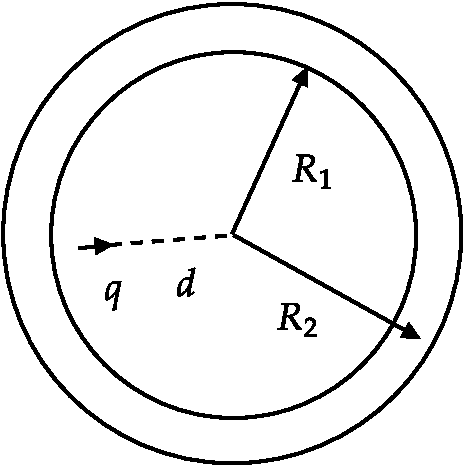
\includegraphics[width=0.22\textwidth]{EM-25-crop}
		\end{center}
	\end{figure}
	\begin{tasks}(4)
		\task[\textbf{a.}] Zero
		\task[\textbf{b.}] $\frac{1}{4 \pi \varepsilon_{0}} \frac{q}{d}$
		\task[\textbf{c.}] $\frac{1}{4 \pi \varepsilon_{0}}\left(\frac{q}{d}-\frac{q}{R_{1}}\right)$
		\task[\textbf{d.}] $\frac{1}{4 \pi \varepsilon_{0}}\left(\frac{q}{d}-\frac{q}{R_{1}}+\frac{q}{R_{2}}\right)$
	\end{tasks}
\item   Consider a spherical dielectric material of radius ' $a$ ' centered at origin. If the polarization vector, $\vec{P}=P_{0} \hat{e}_{x},$ where $P_{0}$ is a constant of appropriate dimensions, then\\ $\left(\hat{e}_{x}, \hat{e}_{y},\right.$ and $\hat{e}_{z}$ are unit vectors in Cartesian- coordinate system){\exyear{IIT JAM 2016}}
\begin{tasks}(1)
	\task[\textbf{a.}] The bound volume charge density is zero.
	\task[\textbf{b.}] The bound surface charge density is zero at $(0,0, a)$.
	\task[\textbf{c.}] The electric field is zero inside the dielectric
	\task[\textbf{d.}] The sign of the surface charge density changes over the surface.
\end{tasks}
	\item An arbitrarily shaped conductor encloses a charge $q$ and is surrounded by a conducting hollow sphere as shown in the figure. Four different regions of space 1,2,3 and 4 are indicated in the figure. Which one of the following statements is correct? {\exyear{IIT JAM 2016}}
	\begin{figure}[H]
		\begin{center}
			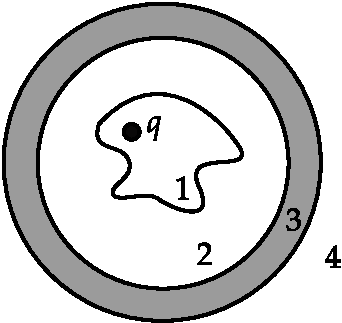
\includegraphics[width=0.22\textwidth]{EM-40-crop}
		\end{center}
	\end{figure}
	\begin{tasks}(1)
		\task[\textbf{a.}] The electric field lines in region 2 are not affected by the position of the charge $q$
		\task[\textbf{b.}] The surface charge density on the inner wall of the hollow sphere is uniform
		\task[\textbf{c.}] The surface charge density on the outer surface of the sphere is always uniform irrespective of the position of charge $q$ in region 1
		\task[\textbf{d.}] The electric field in region 2 has a radial symmetry
	\end{tasks}
	
	

\item For an electric dipole with momentum $\vec{P}=p_{0} \hat{e}_{z}$ placed at the origin, $\left(p_{0}\right.$ is a constant of appropriate dimensions and $\hat{e}_{x}, \hat{e}_{y}$ and $\hat{e}_{z}$ are unit vectors in Cartesian coordinate system){\exyear{IIT JAM 2016}} 
\begin{tasks}(1)
	\task[\textbf{a.}] Potential falls as $\frac{1}{r^{2}},$ where $r$ is the distance from origin
	\task[\textbf{b.}] A spherical surface centered at origin is an equipotential surface
	\task[\textbf{c.}] Electric flux through a spherical surface enclosing the origin is zero
	\task[\textbf{d.}] Radial component of $\vec{E}$ is zero on the $x y-$ plane.
\end{tasks}
\item A unit cube made of a dielectric material has a polarization $\vec{P}=3 \hat{i}+4 \hat{j}$ units. The edges of the cube are parallel to the Cartesian axes. Which of the following statements are true? {\exyear{IIT JAM 2016}}
\begin{tasks}(1)
	\task[\textbf{a.}] The cube carries a volume bound charge of magnitude 5 units.
	\task[\textbf{b.}] There is a charge of magnitude 3 units on both the surfaces parallel to the $y-z$ plane.
	\task[\textbf{c.}] There is a charge of magnitude 4 units on both the surfaces parallel to the $x-z$ plane.
	\task[\textbf{d.}] There is a net non-zero induced charge on the cube.
\end{tasks}

\item For a point dipole of dipole moment $\vec{p}=p \hat{z}$ located at the origin, which of the following is (are) correct? {\exyear{IIT JAM 2017}}
\begin{tasks}(1)
	\task[\textbf{A.}] The electric field at $(0, b, 0)$ is zero
	\task[\textbf{B.}] The work done in moving a charge $q$ from $(0, b, 0)$ to $(0,0, b)$ is $\frac{q p}{4 \pi \epsilon_{0} b^{2}}$
	\task[\textbf{C.}] The electrostatic potential at $(b, 0,0)$ is zero
	\task[\textbf{D.}] If a charge $q$ is kept at $(0,0, b)$ it will exert a force of magnitude $\frac{q p}{4 \pi \in_{0} b^{3}}$ on the dipole.
\end{tasks}
\item A dielectric sphere of radius $R$ has constant polarization $\vec{P}=P_{0} \hat{z},$ so that the field inside the sphere is $\vec{E}_{i n}=-\frac{P_{0}}{3 \epsilon_{0}} \hat{z} .$ Then, which of the following is (are) correct?{\exyear{IIT JAM 2017}}
\begin{tasks}(1)
	\task[\textbf{a.}] The bound surface charge density is $P_{0} \cos \theta$.
	\task[\textbf{b.}] The electric field at a distance $r$ on the $z$ - axis varies as $\frac{1}{r^{2}}$ for $r>>R$.
	\task[\textbf{c.}] The electric potential at a distance $2 R$ on the $z$ - axis is $\frac{P_{0} R}{12 \epsilon_{0}}$.
	\task[\textbf{d.}] The electric field outside is equivalent to that of a dipole at the origin.
\end{tasks}

\colorlet{ocre1}{ocre!70!}
\colorlet{ocrel}{ocre!30!}
\setlength\arrayrulewidth{1pt}
\begin{table}[H]
	\centering
	\arrayrulecolor{ocre}
	\begin{tabular}{|p{1.5cm}|p{1.5cm}||p{1.5cm}|p{1.5cm}|}
		\hline
		\multicolumn{4}{|c|}{\textbf{Answer key}}\\\hline\hline
		\rowcolor{ocrel}Q.No.&Answer&Q.No.&Answer\\\hline
		1&\textbf{d} &2&\textbf{a}\\\hline 
		3&\textbf{d} &4&\textbf{a},\textbf{b} and \textbf{d} \\\hline
		5&\textbf{c} &6&\textbf{a},\textbf{c} and \textbf{d}\\\hline
		7&\textbf{b} and \textbf{c}&8&\textbf{b} and \textbf{c}\\\hline
		9&\textbf{a} ,\textbf{c} and \textbf{d}& & \\\hline
		\end{tabular}
\end{table}
\end{enumerate}
\newpage 
\begin{abox}
Practise Set-2
\end{abox}
\begin{enumerate} [label=\color{ocre}\textbf{\arabic*.}]
	\item  Four point charges are placed in a plane at the following positions:
	$+Q$ at $(1,0),-Q$ at $(-1,0)+Q$ at $(0,1)$ and $-Q$ at $(0,-1)$
	At large distances the electrostatic potential due to this charge distribution will be dominated by the,
	\begin{tasks}(2)
		\task[\textbf{a.}]Monopole moment.  
		\task[\textbf{b.}]Dipole moment.
		\task[\textbf{c.}]Quadrupole moment. 
		\task[\textbf{d.}]Octopole moment. 
	\end{tasks}
\item Three point charges $q, q$ and $-2 q$ are located at $(0,-a, a),(0, a, a)$ and $(0,0,-a)$ respectively.
The net dipole moment of this charge distribution is,
\begin{tasks}(4)
	\task[\textbf{a.}] $4 q a \hat{k}$  
	\task[\textbf{b.}]$2 q a \hat{k}$
	\task[\textbf{c.}] $-4 q a \hat{i}$
	\task[\textbf{d.}]$-2 q a \hat{j}$ 
\end{tasks}
\item Four charges are placed at the four corners of a square of side $a$ as shown in the figure. The electric dipole moment of this configuration is,
\begin{figure}[H]
	\begin{center}
		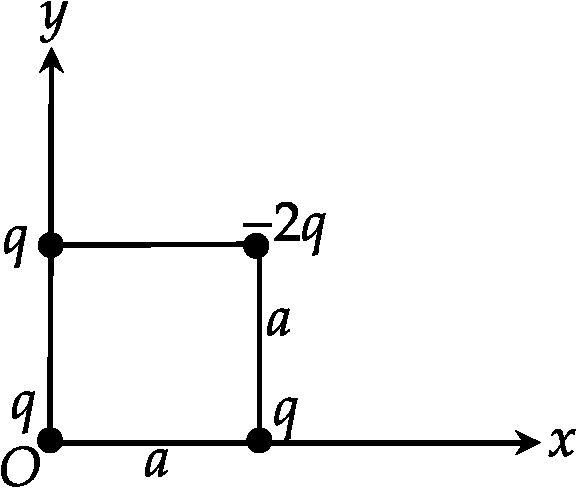
\includegraphics[width=0.25\textwidth]{electric dipole pset-3-6}
	\end{center}
\end{figure}
\begin{tasks}(2)
	\task[\textbf{a.}] $\vec{p}=q a \hat{i}+q \hat{a} \hat{j}$  
	\task[\textbf{b.}]$\vec{p}=-q a \hat{i}+q a \hat{j}$
	\task[\textbf{c.}]$\vec{p}=-q a \hat{i}-q a \hat{j}$ 
	\task[\textbf{d.}]$\vec{p}=q a \hat{i}-q a \hat{j}$	  
\end{tasks}
\item A sphere of radius $R$ carries a polarization $\vec{P}=k \vec{r}$, where $k$ is a constant and $\vec{r}$ is measured
from the centre of the sphere. The bound surface and volume charge densities are given,respectively, by,
\begin{tasks}(4)
	\task[\textbf{a.}] $-k|\vec{r}|$ and $3 k$  
	\task[\textbf{b.}]$k|\vec{r}|$ and $-3 k$
	\task[\textbf{c.}] $k|\vec{r}|$ and $-4 \pi k r$
	\task[\textbf{d.}]  $k|\vec{r}|$ and $4 \pi k r$
\end{tasks}
\item A sphere of radius $R$ carries a polarization $\vec{P}=k \vec{r}$, where $k$ is a constant and $\vec{r}$ is measured
from the centre of the sphere. The electric field $\vec{E}$ at a point $\vec{r}$ outside the sphere is given
by
\begin{tasks}(2)
	\task[\textbf{a.}] $\vec{E}=0$ 
	\task[\textbf{b.}] $\vec{E}=\frac{k R\left(R^{2}-r^{2}\right)}{\varepsilon_{0} r^{3}} \hat{r}$
	\task[\textbf{c.}]  $\vec{E}=\frac{k R\left(R^{2}-r^{2}\right)}{\varepsilon_{0} r^{5}} \hat{r}$
	\task[\textbf{d.}] $\vec{E}=\frac{-k r}{\varepsilon_{0}} \hat{r}$
\end{tasks}
\item Which of the following statements are incorrect?
\begin{tasks}(1)
	\task[\textbf{a.}] The conductivities of conductors and insulators varies with temperature and frequency.
	\task[\textbf{b.}]A conductor is an equipotential body and $\vec{E}$ is allways tangential to the conductor.
	\task[\textbf{c.}] Nonpolar molecules have no permanent dipoles.
	\task[\textbf{d.}] In  linear dielectrics, P varies linearly with E.
\end{tasks}
\item If $\vec{E(r)}=cr\vec{r}$ represents a statics electric field, where c is a constant.Then the charge density of the system is.
\begin{tasks}(4)
	\task[\textbf{a.}] $cr$  
	\task[\textbf{b.}]$3cr$ 
	\task[\textbf{c.}] $5cr$ 
	\task[\textbf{d.}]  $4cr$ 
\end{tasks}
\item A dielectric slab is placed in an electric field. Which of the following statements are correct?
\begin{enumerate}[label=\Roman*.]
	\item  Gauss law can be applied to polarization of charges.
	\item The electric field strength get altered inside the dielectric.\item Polarization charge appears on it's faces.
\end{enumerate}
\begin{tasks}(4)
	\task[\textbf{a.}]II, III only.   
	\task[\textbf{b.}]III only.
	\task[\textbf{c.}]I, II only. 
	\task[\textbf{d.}]I,II, III.  
\end{tasks}
 
 \item  Two dielectrics with dielectric constants $\kappa_{1}$ and $\kappa_{2}$ each fill half the space between the plates of a parallel-plate capacitor as shown in Figure . Each plate has an area $A$ and the plates are separated by a distance $d$. Compute the capacitance of the system.
 \begin{figure}[H]
 	\centering
 	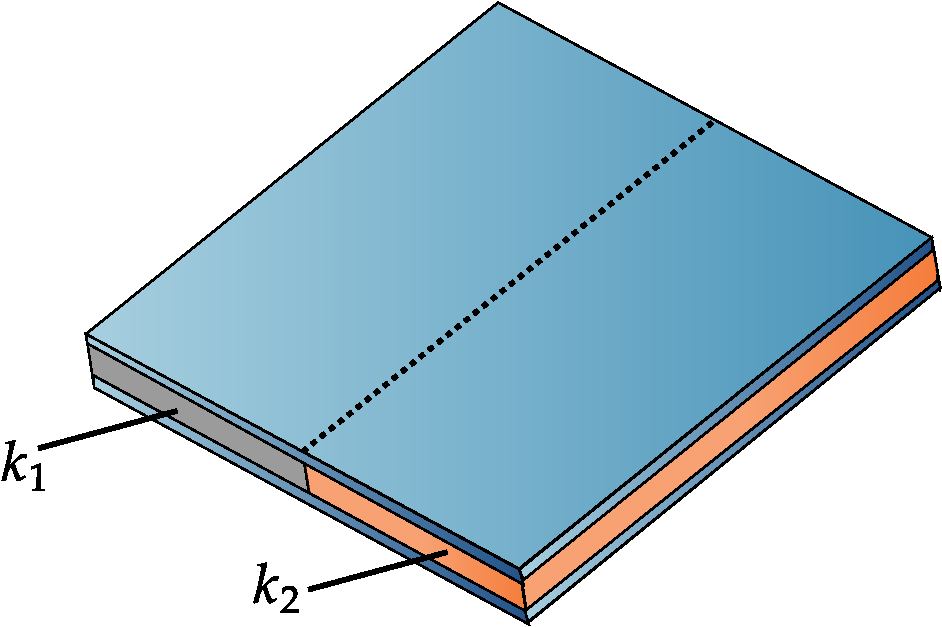
\includegraphics[height=3cm,width=4cm]{pset-2 capacitor}
 	\label{pset-2 capacitor}
 \end{figure}
  \begin{tasks}(4)
 	\task[\textbf{a.}]$\frac{\varepsilon_{0} A}{2 d}\left(\kappa_{1}+\kappa_{2}\right)$
 	\task[\textbf{b.}]$\frac{\varepsilon_{0} A}{2 }\left(\kappa_{1}+\kappa_{2}\right) $
 	\task[\textbf{c.}]$\frac{\varepsilon_{0} A}{4 d}\left(2\kappa_{1}+2\kappa_{2}\right) $
 	\task[\textbf{d.}]$\frac{\varepsilon_{0} A}{2 d}\left(\frac{1}{2}\kappa_{1}+\frac{1}{2}\kappa_{2}\right) $
 \end{tasks} 
\item Consider an air-filled parallel-plate capacitor with one plate connected to a spring having a force constant $k$, and another plate held fixed. The system rests on a table top as shown in Figure . If the charges placed on plates $a$ and $b$ are $+Q$ and $-Q$, respectively, how much does the spring expand?
\begin{figure}[H]
	\centering
	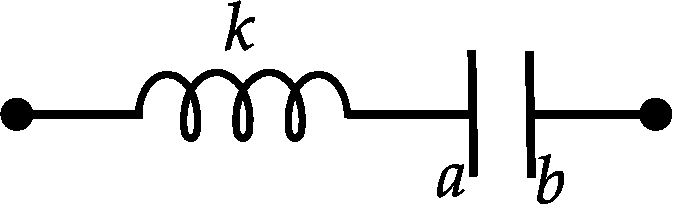
\includegraphics[height=1cm,width=4cm]{capcitor 2 pset-2}
	\label{capcitor 2 pset-2}
\end{figure}
\begin{tasks}(2)
	\task[\textbf{a.}]  $\frac{Q}{2 k A \varepsilon_{0}}$
	\task[\textbf{b.}]  $\frac{Q^{2}}{k A \varepsilon_{0}}$
	\task[\textbf{c.}]  $\frac{Q^{2}}{2 k A \varepsilon_{0}}$
	\task[\textbf{d.}]  $\frac{Q^{3}}{ k A \varepsilon_{0}}$
\end{tasks}
\end{enumerate}
\colorlet{ocre1}{ocre!70!}
\colorlet{ocrel}{ocre!30!}
\setlength\arrayrulewidth{1pt}
\begin{table}[H]
	\centering
	\arrayrulecolor{ocre}
	\begin{tabular}{|p{1.5cm}|p{1.5cm}||p{1.5cm}|p{1.5cm}|}
		\hline
		\multicolumn{4}{|c|}{\textbf{Answer key}}\\\hline\hline
		\rowcolor{ocrel}Q.No.&Answer&Q.No.&Answer\\\hline
		1&\textbf{b} &2&\textbf{a}\\\hline 
		3&\textbf{c} &4&\textbf{b} \\\hline
		5&\textbf{a} &6&\textbf{b} \\\hline
		7&\textbf{d}&8&\textbf{d}\\\hline
		9&\textbf{a}&10&\textbf{c}\\\hline
		
		
	\end{tabular}
\end{table}

\newpage 
\begin{abox}
	Practise Set-3
\end{abox}
\begin{enumerate} [label=\color{ocre}\textbf{\arabic*.}]
		\item  Two capacitors of capacitances $C_{1}$ and $C_{2}$ carrying charges $q_{1}$ and $q_{2}$, respectively, are connected in parallel. A spark appears when the connection is made. Find the energy dissipated by this spark if no other energy dissipation is taking place.
	\begin{answer}
		The total electrostatic energy of the two capacitors before connection is.
		$$
		U_{\text {before }}=\frac{1}{2} \frac{q_{1}^{2}}{C_{1}}+\frac{1}{2} \frac{q_{2}^{2}}{C_{2}}
		$$
		hence the total capacitance of the two capacitors connected in parallel is equal to to the sum of the individua capacitances and since the total charge are connection is equal to the sum of the original charges, the electrostatic energy after connection is
		$$
		U_{\text {after }}=\frac{1}{2} \frac{\left(q_{1}+q_{2}\right)^{2}}{C_{1}+C_{2}}
		$$
		the principle of the conservation of energy, the energy lost in the spark is then
		$$
		U_{\text {spark }}=U_{b}-U_{a}=\frac{1}{2} \frac{q_{1}^{2}}{C_{1}}+\frac{1}{2} \frac{q_{2}^{2}}{C_{2}}-\frac{1}{2} \frac{\left(q_{1}+q_{2}\right)^{2}}{C_{1}+C_{2}}
		$$
		which after simplification becomes,
		$$
		U_{s p a r k}=\frac{1}{2} \frac{\left(C_{1} q_{2}-C_{2} q_{1}\right)^{2}}{2 C_{1} C_{2}\left(C_{1}+C_{2}\right)}
		$$
	\end{answer}
	\item A parallel plate capacitor consist of two plates of area $A$ and plates separated by distance $d$. If space between the plate is filled with a non-uniform dielectric whose dielectric constant varies linearly from value $k_{1}$ at one plate to the value $k_{2}$ at other plate. Then find the capacitance of capacitor.
	\begin{answer}
		Let the dielectric constant at $P$ at a distance $x$ from the plate 1 be $k$ and $\alpha$
		
		\begin{align*}
		\frac{d k}{d x}=\alpha \\
		d k=\alpha d x \\
		k=\alpha x+\beta
		\end{align*}
		Now, at $x=0, k=k_{1}$ and at $x={d}, k=k_{2}$
		\\$k=\frac{\left(k_{2}-k_{1}\right) x}{d}+k_{1}$
		Now the the field at $P$ is
		\begin{align*}
		E &=\frac{\sigma}{\varepsilon}=\frac{\sigma}{\varepsilon_{0} k}=\frac{\sigma}{\varepsilon_{0}\left[\frac{\left(k_{2}-k_{1}\right) x}{d}+k_{1}\right]} \\
		V &=-\int_{d}^{0} E d x=\frac{\sigma}{\varepsilon_{0}} \int_{0}^{d} \frac{d x}{\left.\left(k_{2}-k_{1}\right) x_{1}\right)_{1}} \frac{\sigma_{1}}{d} \\
		&=\left.\frac{\sigma d}{\varepsilon_{0}\left(k_{2}-k_{1}\right)} \ln \left(\frac{k_{2}-k_{1}}{d} x+k_{1}\right)\right|_{0} ^{d}\\
		&=\frac{\sigma d}{\varepsilon_{0}\left(k_{2}-k_{1}\right)} \ln \left(\frac{k_{2}-k_{1}+k_{1}}{k_{1}}\right)\\&=\frac{Q d}{\varepsilon_{0} A\left(k_{2}-k_{1}\right)} \ln \left(\frac{k_{2}}{k_{1}}\right) \\
		c&=\frac{Q}{V}=\frac{\varepsilon_{0} A}{d} \frac{\left(k_{2}-k_{1}\right)}{\ln \left(k_{2} / k_{1}\right)}
		\end{align*}
	\end{answer}
	\item The conductors in a $0.75 \mathrm{~km}$ long two-wire transmission line are separated by a centre-to-centre distance of $0.2 \mathrm{~m}$. If each conductor has a diameter of $4 \mathrm{~cm}$, then the capacitance of the line is
	\begin{tasks}(2)
		\task[\textbf{a.}]$8.85 \mu \mathrm{F}$  
		\task[\textbf{b.}]$88.5 \mathrm{nF}$
		\task[\textbf{c.}]$8.85 \mathrm{pF}$ 
		\task[\textbf{d.}]$8.85 \mathrm{nF}$ 
	\end{tasks}
	
	\begin{answer}
		(derive capacitance of two wire capacitors)
	\end{answer}
	\item Consider a parallel plate capacitor with plate separation $d$ and each plate having a length $l$ and width $a$. A dielectric slab of permittivity $\in$, thickness $\mathrm{d}$, length $l$ and width $a$ is partially inserted between the plates. If a constant $\mathrm{pd} \mathrm{V}$ is maintained between the plates, find the force exerted on the dielectric slab when a length $x$ of the slab remains between the plates.
	The system may be considered as the parallel combination of two capacitors $\mathrm{C}_{1}$ and $\mathrm{C}_{2}$, where, The total capacitance is then
	The electrostatic energy of the system is
	\begin{answer}
		$$
		U=\frac{1}{2} C V^{2}=\frac{a}{2 d}\left[\left(\in-\epsilon_{0}\right) x+\epsilon_{0} \ell\right] V^{2}
		$$
		As $V$ is constant the force experienced by the slab will be
		$$
		\vec{F}=\left.\frac{\partial U}{\partial x}\right|_{V} \hat{x}=\frac{a}{2 d}\left(\epsilon-\epsilon_{0}\right) V^{2} \hat{x}
		$$
		where $\hat{x}$ is a unit vector in the direction of increasing $x .$ This means that the force is attractive.
	\end{answer}
	
	\item 	 A "pure" dipole $\vec{p}$ is situated at the origin, pointing in the $z$ -direction
	\\(a) What is the force on a point charge $q$ at $(a, 0,0)$ ?
	\\(b) What is the force on $q$ at $(0,0, a)$ ?
	\\(c) How much work does it take to move $q$ from $(a, 0,0)$ to $(0,0, a)$ ?
	\begin{answer}\hspace{0.5cm}
	\begin{enumerate}
		\item \begin{align*}
			 A t(a, 0,0), r&=a, \theta=\frac{\pi}{2} ; \\\vec{E}&=\frac{p}{4 \pi \varepsilon_{0} r^{3}}(2 \cos \theta \hat{r}+\sin \theta \hat{\theta})=\frac{p}{4 \pi \varepsilon_{0} a^{3}} \hat{\theta} \\
			\vec{E}&=-\frac{p}{4 \pi \varepsilon_{0} a^{3}} \hat{z} \Rightarrow \vec{F}=q \vec{E}=-\frac{p q}{4 \pi \varepsilon_{0} a^{3}} \hat{z}
			\end{align*}
			\item \begin{align*}
				A t(0,0, a), r&=a, \theta=0 ;\\ \vec{E}&=\frac{p}{4 \pi \varepsilon_{0} r^{3}}(2 \cos \theta \hat{r}+\sin \theta \hat{\theta})=\frac{2 p}{4 \pi \varepsilon_{0} a^{3}} \hat{r} \\
			\vec{E}&=\frac{2 p}{4 \pi \varepsilon_{0} a^{3}} \hat{z} \Rightarrow \vec{F}=q \vec{E}=\frac{2 p q}{4 \pi \varepsilon_{0} a^{3}} \hat{z}
			\end{align*}
			\item \begin{align*}
				 V_{d i p}(r, \theta)&=\frac{p \cos \theta}{4 \pi \varepsilon_{o} r^{2}} \Rightarrow V(a, 0,0)=0 \text { and } V(0,0, a)=\frac{p}{4 \pi \varepsilon_{o} a^{2}}, \\
			W&=q[V(0,0, a)-V(a, 0,0)]=\frac{p}{4 \pi \varepsilon_{o} a^{2}}
			\end{align*}
	\end{enumerate}
	
	\end{answer}
\item The electric field at a point due to an electric dipole is perpendicular to the dipole axis, the
angle between the dipole axis and the line joining the point with the centre of the dipole
is $\tan ^{-1}(\beta)$. Then the value of $\beta$ is $\ldots \ldots$.
\begin{answer}


	\begin{align*}
	\vec{E}(r, \theta)&=\frac{p}{4 \pi \varepsilon_{0} r^{3}}(2 \cos \theta \hat{r}+\sin \theta \hat{\theta}) \\
	\tan \alpha&=\frac{E_{\theta}}{E_{r}}=\frac{1}{2} \tan \theta \quad \because \alpha=90-\theta \Rightarrow \cot \theta=\frac{1}{2} \tan \theta \\
	\Rightarrow \tan ^{2} \theta&=2 \Rightarrow \theta=\tan ^{-1} \sqrt{2}
	\end{align*}
	
\end{answer}
\item Let four point charges $q,-q / 2, q$ and $-q / 2$ be placed at the vertices of a square of
side $a$. Let another point charge $-q$ be placed at the cnetre of the square (see the figure).
Let $V(r)$ be the electrostatic potential at a point $P$ at a distance $r \gg a$ from the centre of
the square. Then $V(3 r) / V(r)$ is.....................
\begin{answer} the monopole moment,\\
	  $Q_{\text {mono }}=-\frac{q}{2}+q-\frac{q}{2}+q-q=0$
   \begin{align*}
	\vec{p}&=q(a \hat{x}+a \hat{y})-\frac{q}{2}(a \hat{x}+a \hat{y})-q(a \hat{x}-a \hat{y})+q(-a \hat{x}-a \hat{y})-\frac{q}{2}(-a \hat{x}+a \hat{y})+0=0 \\
	\text { Thus } V &\propto \frac{1}{r^{3}} \Rightarrow \frac{V(3 r)}{V(r)}=\frac{1}{27}=0.037
	\end{align*}
	
\end{answer}
\item A "pure" dipole with dipole moment $\vec{p}=p_{o} \hat{z}$ is situated at the origin. A point charge $Q$ is
moved from the point $(\mathrm{a}, 0,0)$ to $(0,0, \mathrm{a})$ then the work done will be,
\begin{tasks}(4)
	\task[\textbf{a.}]  zero. 
	\task[\textbf{b.}]$\frac{p_{0} Q}{4 \pi \varepsilon_{0} a^{3}}$
	\task[\textbf{c.}] $\frac{p_{0}}{4 \pi \varepsilon_{0} a^{2}}$
	\task[\textbf{d.}] $\frac{p_{0} Q}{4 \pi \varepsilon_{0} a^{2}}$
\end{tasks}
\begin{answer}
	\begin{align*}
    W&=Q[V(0,0, a)-V(a, 0,0)]\\
	V(r, \theta)&=\frac{p_{0} \cos \theta}{4 \pi \varepsilon_{0} r^{2}}\\ \Rightarrow V(0,0, a)&=\frac{p_{0}}{4 \pi \varepsilon_{0} a^{2}} \quad \because \theta=0 \text { and } V(a, 0,0)=0 \quad \because \theta=\frac{\pi}{2}\\
	\Rightarrow W&=\frac{p_{0} Q}{4 \pi \varepsilon_{0} a^{2}}
	\end{align*}
	
\end{answer}

\end{enumerate}




